% !TeX root = orbits.tex

\chapter{The Two Definitions of an Ellipse}\label{s.two-defs}

Ellipses were defined in two ways (Figure~\ref{f.two-defs}).

\textbf{Definition~\ref{def.ellipse1}:} 
Given $S$ and $S'$,\footnote{To be consistent with \cite{besant} the second focus is labeled $S'$ and not $H$.} two points (the \emph{foci}) such that $SS'=2c>0$, and $2a>2c>0$, an \emph{ellipse} is the locus of points $P$ such that $SP+PS'=2a$ (red). The \emph{eccentricity} is $c/a$.

\textbf{Definition~\ref{def.ellipse2}:} 
Given a line (the \emph{directrix}), a point $S$ (a \emph{focus}) at distance $SX=d>0$ from the directrix and $0<e<1$ (the \emph{eccentricity}), an \emph{ellipse} is the locus of points $P$ such that $SP/PK=e$ (blue). $A$ on $SX$ is a \emph{vertex} of the ellipse if $SA/AX=e$.

In Section~\ref{s.parameters} we show how to compute the parameters $a$ and $c$ of Definition~\ref{def.ellipse1} from $d$ and $e$ of Definition~\ref{def.ellipse2}. Computing $d$ from $a$ and $e$ follows immediately.

Section~\ref{s.2a} proves in Euclidean geometry that $SP+PS'$ is equal to $AA'$, the major axis of length $2a$, when the directrix and $e$ are given according to Definition~\ref{def.ellipse2}. 

\section{Computing the parameters of the definitions}\label{s.parameters}

%%%%%%%%%%%%%%%%%%%%%%%%%%%%%%%%%%%%%%%%%%%%

\begin{figure}[b]
\begin{center}
\begin{tikzpicture}
% Ellipse
\def\a{3.75}
\def\b{2.5}
\pic{ellipse={{\a}/{\b}}};

% Label nodes
\node[above] at (Top) {$B$};

\node[below right] at (Right) {$A'$};
\node[below left] at (Left) {$A$};
\node[below] at (F1) {$S$};
\node[below] at (F2) {$S'$};
\node[below left,xshift=3pt,yshift=-2pt] at (O) {$O$};

% Label segments
\path (Top) --  node[right,near start] {$b$} (O);
\path (F1) -- node[below] {$c$} (O) -- node[below] {$c$} (F2);
\draw (F1) -- node[below] {$a$} (Top);
\draw (O) rectangle +(6pt,6pt);

\def\x{3.75+sqrt(5)}
\coordinate (X) at ({-(\x)},0);
\node[below left] at (X) {$X$};
\draw (Left) -- (X) -- +(0,{\b});
\draw (X) -- +(0,{-\b});

% Indicates distances along the major axis
\draw[<->] ($(O)+(0,-20pt)$) -- node[fill=white] {$a$} ($(Right)+(0,-20pt)$);
\draw[<->] ($(O)+(0,-20pt)$) -- node[fill=white] {$a$} ($(Left)+(0,-20pt)$);
\draw[<->] ($(X)+(0,-40pt)$) -- node[fill=white] {$d$} ($(F1)+(0,-40pt)$);

\def\angle{120}
\coordinate (P) at ({\angle}:{\a} and {\b});
\path[name path global=fromF1p] (P) -- (F1);
\path[name path=ph] (P) -- (F2);
\path[name path global=pc] (P) -- (O);
\node[above left] at (P) {$P$};
\draw[thick,red] (F1) -- (P) -- (F2);

\draw[thick,blue] ($(F1)+(-2pt,0)$) -- ($(P)+(-2pt,0)$);
\draw[thick,blue] ($(P)+(-2pt,0)$)  -- (P -| X) coordinate (K);
\node[left] at (K) {$K$};
\draw[blue,rotate=-90] (K) rectangle +(6pt,6pt);

\end{tikzpicture}
\caption{Two definitions of an ellipse}
\label{f.two-defs}
\end{center}
\end{figure}

%%%%%%%%%%%%%%%%%%%%%%%%%%%%%%%%%%%%%%%%%%%%%%%%%%%%%%%%%%

$AX$ and $A'X$ can be computed from $d$ and $e$.
\begin{eqnlabels}
SA+AX&=&SX=d\nonumber\\[4pt]
SA&=&d-\frac{SA}{e}=d\cdot \frac{e}{1+e}\label{eqn.sa}\\[4pt]
AX&=&d\cdot \frac{1}{1+e}\nonumber\\[4pt]
A'X-SA'&=&d\nonumber\\[4pt]
SA'&=&\frac{SA'}{e}-d=d\cdot \frac{e}{1-e}\nonumber\\[4pt]
A'X&=&d\cdot \frac{1}{1-e}\nonumber\,.
\end{eqnlabels}%
$a$ can now be computed from $A'X-AX$.
\begin{eqnlabels}
a=\frac{AA'}{2}&=&
\frac{1}{2}( A'X-AX)=
\frac{d}{2}\left(\frac{1}{1-e}-\frac{1}{1+e}\right)\nonumber\\[4pt]
&=&\frac{d}{2}\cdot\frac{2e}{1-e^2}=d\cdot\frac{e}{1-e^2}\,.\label{eqn.a}
\end{eqnlabels}%
$c$ is $a-SA$ so by Equations~\ref{eqn.sa}, \ref{eqn.a},
\[
c=OS=a-SA=
d\cdot\frac{e}{1-e^2} - d\cdot \frac{e}{1+e}=d\cdot \frac{e^2}{1-e^2}\,.
\]%
Finally, $b$ can be computed as $\sqrt{a^2-c^2}$.
\[
b=
d\cdot\sqrt{\frac{e^2}{(1-e^2)^2}-\frac{e^4}{(1-e^2)^2}}=
d\cdot\frac{e^2}{1-e^2}\cdot\sqrt{1-e^2}=
d\cdot \frac{e}{\sqrt{1-e^2}}\,.
\]
Conversely, by Equation~\ref{eqn.a}, $d$ can be computed from $a$ and $e$:
\[
d=a\cdot\frac{1-e^2}{e}\,.
\]

As an example, we compute the factors for $e=\sqrt{5}/3$ and then multiply it by various values of $d$.
\begin{eqn}
a/d&=&\frac{e}{1-e^2}=\frac{\sqrt{5}/3}{4/9}=\frac{3\sqrt{5}}{4}\\[4pt]
c/d&=&\frac{e^2}{1-e^2}=\frac{5/9}{4/9}=\frac{5}{4}\\[4pt]
b/d&=&\frac{e}{\sqrt{1-e^2}}=\frac{\sqrt{5}/3}{2/3}=\frac{\sqrt{5}}{2}\,.
\end{eqn}%
For $d=4/\sqrt{5}$ we have:
\[
a=3,\qquad b = 2,\qquad c = \sqrt{5}\,.
\]
Conversely,
\[
d=a\cdot\frac{1-e^2}{e}=3\cdot \frac{4/9}{\sqrt{5}/3}=\frac{4}{\sqrt{5}}\,.
\]

Figure~\ref{f.two-defs} was drawn with $d=\sqrt{5}$ giving:
\[
a=15/4=3.75,\qquad b=5/2 = 2.5,\qquad c = 5\sqrt{5}/4\approx 2.8\,.
\]

\section{The sum of the distances to the foci equals the major axis}\label{s.2a}

\begin{theorem}
In Figure~\ref{f.cacx}, which shows the points on the major axis of an ellipse,
\begin{equation}
\frac{SA}{AX}=\frac{AA'}{XX'}\,.\label{eqn.cacx}
\end{equation}
\end{theorem}

\begin{figure}[ht]
\begin{center}
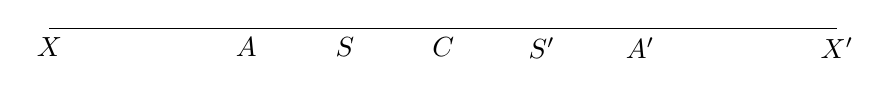
\begin{tikzpicture}[scale=1.25]

\coordinate (X) at (0,0);
\node[below] at (X) {$X$};
\vertexsm{X};
\coordinate (A) at (2,0);
\node[below] at (A) {$A$};
\vertexsm{A};
\coordinate (S) at (3,0);
\node[below] at (S) {$S$};
\vertexsm{S};
\coordinate (C) at (4,0);
\node[below] at (C) {$C$};
\vertexsm{C};
\coordinate (SP) at (5,0);
\node[below] at (SP) {$S'$};
\vertexsm{SP};
\coordinate (AP) at (6,0);
\node[below] at (AP) {$A'$};
\vertexsm{AP};
\coordinate (XP) at (8,0);
\node[below] at (XP) {$X'$};
\vertexsm{XP};

\draw (X) -- (XP);

\end{tikzpicture}
\caption{The major axis of an ellipse}
\label{f.cacx}
\end{center}
\end{figure}

\begin{proof}
From the Figure we see that
\begin{eqn}
\frac{AA'}{SA}-1&=&\frac{AA'}{SA}-\frac{SA}{SA}=
\frac{AA'-SA}{SA}=\frac{SA'}{SA}\\[8pt]
\frac{XX'}{AX}-1&=&\frac{XX'}{AX}-\frac{AX}{AX}=
\frac{XX'-AX}{AX}=\frac{AX'}{AX}\,.
\end{eqn}
But $A,A'$ are both points on the ellipse so
\begin{eqn}
\frac{SA'}{AX'}&=&\frac{SA}{AX}\\[4pt]
\frac{SA'}{SA}&=&\frac{AX'}{AX}\\[4pt]
\frac{AA'}{SA}&=&\frac{XX'}{AX}\,.\fqed
\end{eqn}
\end{proof}

\begin{theorem}
$SP+S'P = AA'$.
\end{theorem}

\begin{figure}[b]
\begin{center}
\begin{tikzpicture}
% Ellipse
\def\a{3}
\def\b{2}
\pic{ellipse={{\a}/{\b}}};

% Label nodes
\node[below right] at (Right) {$A'$};
\node[below left] at (Left) {$A$};
\node[below] at (F1) {$S$};
\node[below] at (F2) {$S'$};
\node[below left,xshift=3pt,yshift=-2pt] at (O) {$O$};

\coordinate (X) at (-4,0);
\node[below left] at (X) {$X$};
\draw (Left) -- (X) -- +(0,{\b});
\draw (X) -- +(0,{-\b});
\coordinate (XP) at (4,0);
\node[below right] at (XP) {$X'$};
\draw (Right) -- (XP) -- +(0,{\b});
\draw (XP) -- +(0,{-\b});

% Indicates distances along the major axis
\draw[<->] ($(O)+(0,-20pt)$) -- node[fill=white] {$a$} ($(Right)+(0,-20pt)$);
\draw[<->] ($(O)+(0,-20pt)$) -- node[fill=white] {$a$} ($(Left)+(0,-20pt)$);

\def\angle{110}
\coordinate (P) at ({\angle}:{\a} and {\b});
\path[name path global=fromF1p] (P) -- (F1);
\path[name path=ph] (P) -- (F2);
\path[name path global=pc] (P) -- (O);
\node[above left] at (P) {$P$};
\draw[thick,red] (F1) -- (P) -- (F2);
\coordinate (N) at (P|-O);
\draw[thick,blue] (P) -- (N) node[below,black] {$N$};
\draw[blue,thick] (N) rectangle +(7pt,7pt);

\draw[thick,dashed] (P-|X) node[left] {$K$} -- (P-|XP) node[right] {$K'$};

\end{tikzpicture}
\caption{$SP+SP'=AA'$}
\label{f.AAP}
\end{center}
\end{figure}

\begin{proof}
Let $N$ be the perpendicular from $P$ to the major axis (Figure~\ref{f.AAP}). $P$ is on the ellipse if $SP/PK=e$ or $SP'/PK'=e$, but since $PK=NX$ and $PK'=NX'$, $P$ is on the ellipse if $SP/NX=e$ or $SP'/NX'=e$.
\begin{eqn}
\frac{SP}{NX}&=&\frac{SP'}{NX'}\\[4pt]
\frac{SP'}{SP}&=&\frac{NX'}{NX}\\[4pt]
\frac{SP'+SP}{SP}&=&\frac{NX'+NX}{NX}\\[4pt]
\frac{SP'+SP}{SP}&=&\frac{XX'}{NX}\,.
\end{eqn}
Again since $P$ is on the ellipse and by Equation~\ref{eqn.cacx},
\begin{eqn}
\frac{SP'+SP}{XX'}&=&\frac{SP}{NX}=\frac{SA}{AX}=\frac{AA'}{XX'}\\[4pt]
SP'+SP&=&AA'\,.\fqed
\end{eqn}
\end{proof}

